\documentclass[aspectratio=169,14pt,usenames,dvipsnames]{beamer}

\usepackage[utf8]{inputenc}
\usepackage{enumitem}
\usepackage{calc}

\usepackage{datetime}
\newcommand\builddate{%
   \ifcase \month%
        \or Janeiro%
        \or Fevereiro%
        \or Março%
        \or Abril%
        \or Maio%
        \or Junho%
        \or Julho%
        \or Agosto%
        \or Setembro%
        \or Outubro%
        \or Novembro%
        \or Dezembro%
    \fi\space\number\year%
}

\newcommand{\loadtheme}[1]{%
    \input{themes/#1}%
}
\newcommand{\presentationlanguage}[1]{%
    \usepackage[#1]{babel}%
}

\newcommand{\usecodingsamples}[1]{%
    \usepackage{listings}%
    \input{listings/#1}%
}

% Configura a apresentação para ser executada em tela cheia.
\newcommand{\setfullscreen}{\hypersetup{pdfpagemode=FullScreen}}

% Hide beamer navigation simbols
\beamertemplatenavigationsymbolsempty

%
% Standard frames
%

% coverframe
\newcommand{\coverframe}{%
    \begin{frame} %
        \titlepage %
    \end{frame} %
}

% finalframe{email}
\newcommand{\finalframe}[2][Thank you!]{%
    \begin{frame}%
        \begin{flushright}%
            \huge \textbf{#1}%
            \vfill%
            \large \textbf{#2}%
        \end{flushright}%
    \end{frame}%
}

\newcommand{\bigtitle}[1]{%
    \begin{frame}%
        \begin{center}%
            \Huge {#1}%
        \end{center}%
    \end{frame}%
}


\usecodingsamples{python}

\loadtheme{invaders}

\title{Desenvolvedo Jogos com PyGame}
\subtitle{}
\author{Rafael Guterres Jeffman}
\institute{Tchelinux}
\date{2018}

\begin{document}

%01
\coverframe


%02
\begin{frame}
    \frametitle{Por que Jogos?}

    \begin{itemize}
        \item Daemon Attack
        \item Pitfall
        \item Enduro
        \item River Raid
        \item Decathlon
    \end{itemize}
\end{frame}

%03
\begin{frame}
    \frametitle{Por que Python?}

    \begin{itemize}
        \item Expressividade
        \item Simplicidade
        \item Multi-paradigma
    \end{itemize}
\end{frame}

%04
\begin{frame}
    \frametitle{Por que PyGame?}

    \begin{itemize}
        \item Abstrai boa parte das "parada chata".
        \item \textit{Cross-platform} (SDL)
        \item Modelo de aplicação simples.
    \end{itemize}
\end{frame}

%04
\begin{frame}
    \frametitle{O que é e não é PyGame?}

    \begin{itemize}
        \item É uma biblioteca que auxilia no desenvolvimento de jogos.
        \item Não é um \textit{engine} de jogos.
        \item É uma coleção de métodos e ferramentas de \textit{baixo nível}.
        \item Não é para desenvolver o novo FPS 3D a 240fps em 4K.
        \item Mas é bacana para desenvolver jogos 2D...
    \end{itemize}
\end{frame}

%05
\begin{frame}[fragile]
    \frametitle{Modelo de Aplicação}

    \begin{python}
        import sys, pygame
        pygame.init()

        # initialize stuff
        while True:
            # handle events
            # update game objects
            # redraw screen stuff
            pygame.display.flip()
    \end{python}
\end{frame}

%04
\begin{frame}
    \frametitle{O Projeto}

    \begin{itemize}
        \item Um diretório \textbf{media} onde serão armazenados os arquivos de
        mídia do jogo, com subdiretórios para sons, imagens, vídeos.
        \item Um diretório \textbf{features}, afinal, você vai usar o
        {\color{blue}\underline{\href{https://github.com/behave}{behave}}}
        \item O seu código, bem organizado...
    \end{itemize}
\end{frame}

%04
\begin{frame}
    \frametitle{\textit{Side Scrolling Shot'em Up}}
    {\large\bfseries
    \begin{center}
        Sua nave foi transportada para o quadrante \textit{gamma}, no meio das hordas
        inimigas, durante a \textit{Guerra do Infinito}.
        \vspace{1cm}

        Sua missão, aceite ou não, é destruir\\todos os inimigos.
    \end{center}
    }
\end{frame}

%04
\begin{frame}[fragile]
    \frametitle{A Tela da Aplicação}

    \begin{itemize}
        \item PyGame utiliza SDL para o gerenciamento da janela.
        \item Deve ser definido o tamanho da janela na sua criação.
        \item \textit{Flags} podem ser utilizados para configurar a tela.
    \end{itemize}

    \begin{python}
        size = width, height = (800, 600)
        flags = pygame.FULLSCREEN
        screen = pygame.display.set_mode(size, flags)
    \end{python}
\end{frame}

%04
\begin{frame}
    \frametitle{Cenários}

    \begin{itemize}
        \item PyGame não tem o conceito de \textit{engine}, logo, o cenário
        também é parte do código.
        \item O cenário pode ser criado a partir de um procedimento.
        \item Mesmo em um ambiente 2D, é possível trazer uma sensação de
        profundidade.
        \item Para criar o efeito de \textit{parallax}, você deve criar planos
        que se movimentam em velocidades diferentes.
    \end{itemize}
\end{frame}

%04
\begin{frame}
    \frametitle{Objetos do Jogo}

    \begin{itemize}
        \item Uma forma de facilitar a escrita do código é criar objetos de jogo.
        \item Estes objetos devem prover métodos para criação, movimentação e
        \textit{rendering}.
        \item Tratar estes objetos com uma lista de objetos básicos simplifica
        o código e não afeta a performance.
    \end{itemize}
\end{frame}

%04
\begin{frame}
    \frametitle{O Protagonista}

    \centering
    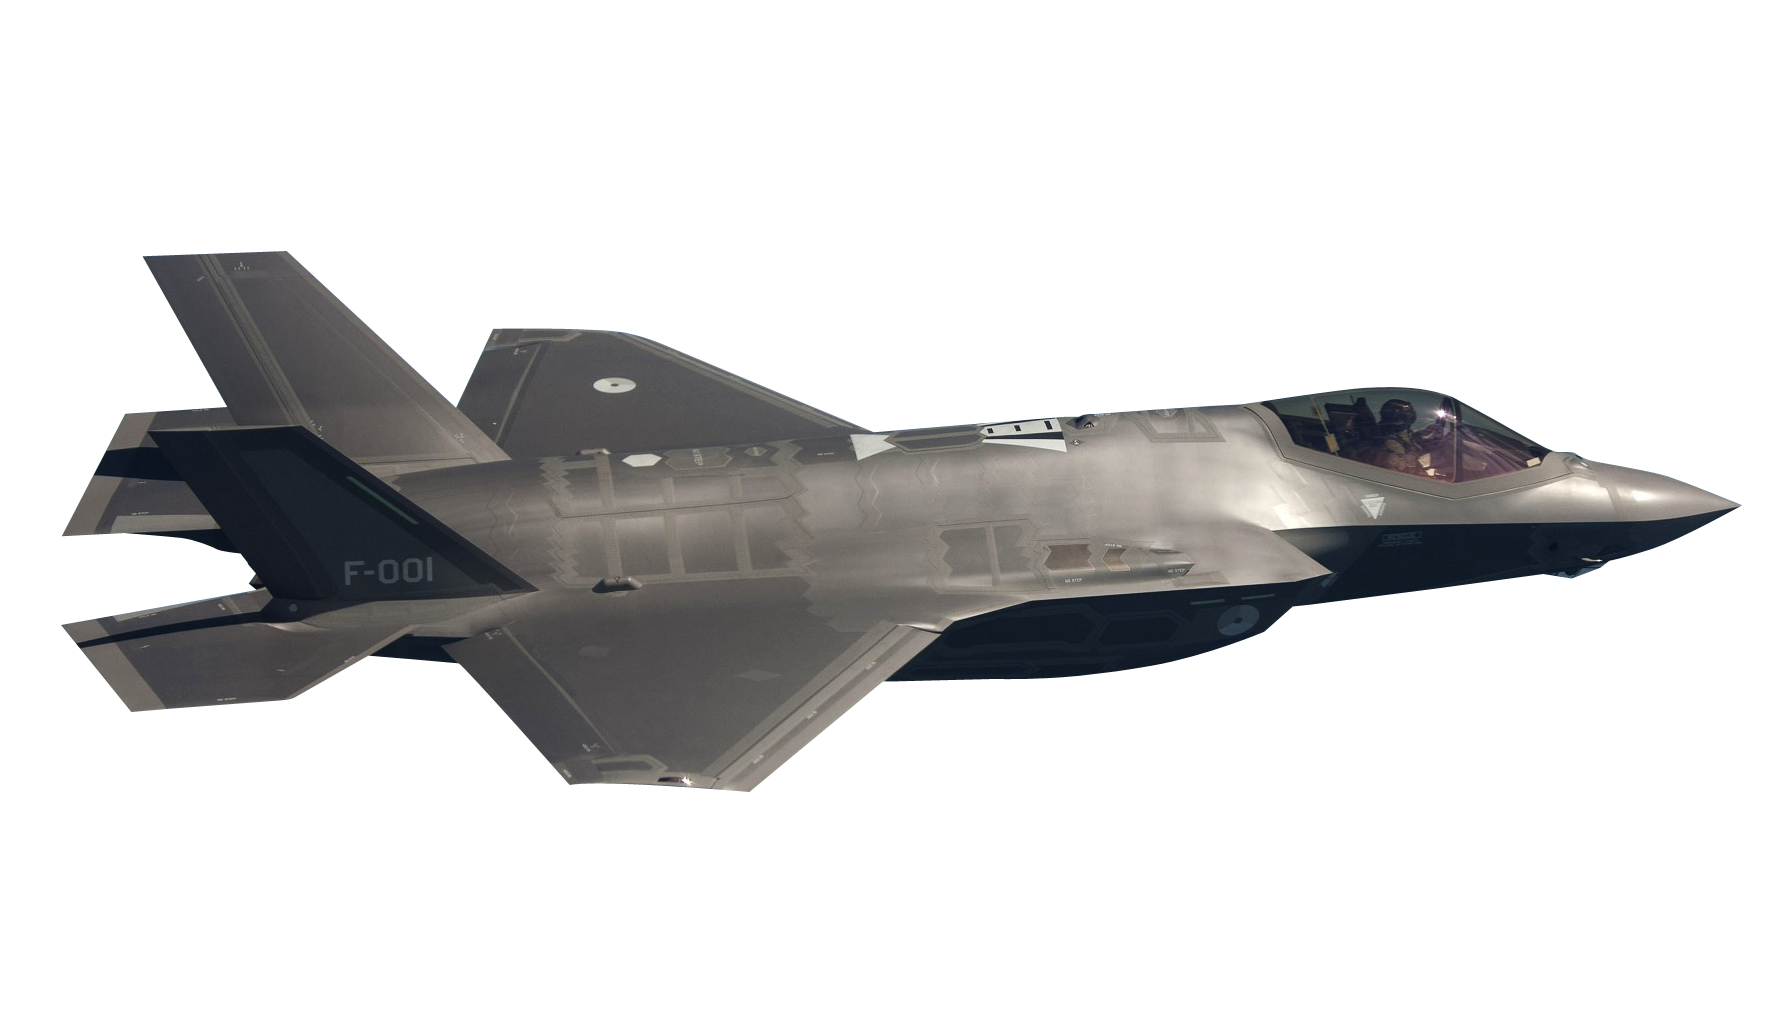
\includegraphics[height=0.7\paperheight]{code/media/images/f18-big.png}
\end{frame}

%04
\begin{frame}
    \frametitle{Controle}

    \begin{itemize}
        \item O controle dos objetos é realizado a partir do loop de eventos.
        \item Os eventos de teclado são divididos em KEYDOWN e KEYUP.
        \item Também estão disponíveis eventos de \textit{mouse} e
        \textit{joystick}.
    \end{itemize}
\end{frame}

\begin{frame}[fragile]
    \frametitle{Mostrando Textos}
    \begin{python}
        # Desnecessário se você usou pygame.init()
        pygame.font.init()

        myfont = pygame.font.SysFont('Lucida Sans', 30)

        textsurface = myfont.render('Lorem Ipsum', False, (0, 0, 0))

        screen.blit(textsurface,(0,0))
    \end{python}
\end{frame}

%04
\begin{frame}
    \frametitle{Quão produtivo é o PyGame?}

    \begin{itemize}
        \item Sem conhecer o PyGame...
        \item Precisando viajar a Pelotas...
        \item Precisando dormir...
        \item Precisando ministrar uma aula...
        \item Precisando criar essa palestras...
        \item Precisando sair com os cachorros...
    \end{itemize}
\end{frame}

\begin{frame}
    \huge\centering
    Em 24h,\\com auxílio da Internet,\\é possível fazer um jogo\\(e essa palestra).
\end{frame}

%04
\begin{frame}
    \frametitle{O Antagonista}

    \centering
    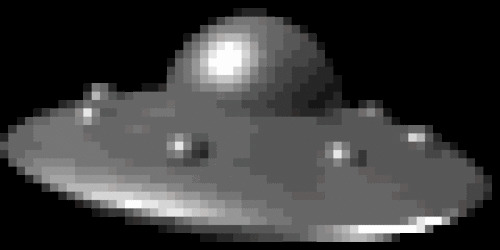
\includegraphics[height=1cm]{code/media/images/ufo_spin-7.jpg}
\end{frame}

%04
\begin{frame}
    \frametitle{E Agora?}
    \centering
    \Huge\url{https://pygame.org}
\end{frame}
%20
\finalframe[Muito Obrigado!]{
    \url{https://rafaeljeffman.com/tchelinux}
    \url{email@example.com}
}

\end{document}
